\documentclass[10pt,letterpaper]{article}
\usepackage{fontspec}
\usepackage{amsmath,amssymb}
\usepackage{graphicx}
\usepackage{xcolor}
\usepackage{tcolorbox}
\tcbuselibrary{skins}
\usepackage{geometry}
\usepackage{booktabs}
\usepackage{colortbl}
\usepackage{fancyhdr}
\usepackage{titlesec}
\usepackage[shortlabels,inline]{enumitem}
\usepackage{tabularx}
\usepackage{array}
\usepackage{multicol}
\usepackage{tikz}

\setmainfont{Times New Roman}
\setsansfont{Arial}

\geometry{
    paperwidth=612.05pt,
    paperheight=720.05pt,
    top=33.8pt,
    headheight=13pt,
    headsep=16pt,
    bottom=44pt,
    footskip=18pt,
    left=36pt,
    right=36pt,
    includehead
}

\definecolor{stewartcyan}{RGB}{0, 118, 186}
\definecolor{stewartred}{RGB}{218, 41, 28}
\definecolor{stewarttableheader}{RGB}{210, 224, 238}
\definecolor{stewarttablehead}{RGB}{210, 224, 238}
\definecolor{tableblue}{RGB}{210, 224, 238}
\definecolor{stewartlightblue}{RGB}{235, 243, 250}
\definecolor{stewartblue}{RGB}{0, 118, 186}
\definecolor{stewartgray}{RGB}{120, 120, 120}
\definecolor{stewartlightgray}{RGB}{240, 240, 240}
\definecolor{stewartpurple}{RGB}{85, 30, 95}
\definecolor{stewartpurplebg}{RGB}{243, 238, 245}
\definecolor{stewartpurpletext}{RGB}{85, 30, 95}
\definecolor{darkgray}{RGB}{40, 40, 40}

\pagestyle{fancy}
\fancyhf{}
\renewcommand{\headrulewidth}{0pt}

\providecommand{\makecell}[2][c]{\begin{tabular}[#1]{@{}c@{}}#2\end{tabular}}
\providecommand{\faDesktop}{\textbf{[Máy tính]}}
\providecommand{\casicon}{\textbf{\textsf{[CAS]}}}
\providecommand{\ticon}{\textbf{\textsf{[T]}}}
\providecommand{\captionof}[2]{\par\vspace{2pt}{\small\textbf{#1}: #2}\par}
\NewDocumentEnvironment{tasks}{o d()}{\begin{enumerate}}{\end{enumerate}}
\providecommand{\task}{\item}
\newenvironment{redframebox}{\begin{definitionbox}}{\end{definitionbox}}

\newtcolorbox{definitionbox}{
    colback=white,
    colframe=stewartred,
    arc=0mm,
    boxrule=0.9pt,
    left=3.5mm, right=3.5mm, top=3mm, bottom=3mm
}

\begin{document}
\begin{minipage}[t]{0.485\textwidth}

    \noindent
    \textbf{\textsf{\color{stewartcyan}39--46}}\quad Tìm tập xác định của hàm số.

    \vspace{0.33em}
    \noindent
    \begin{minipage}[t]{0.48\textwidth}
        \textbf{39.} $f(x) = \dfrac{x + 4}{x^2 - 9}$
    \end{minipage}%
    \hfill
    \begin{minipage}[t]{0.48\textwidth}
        \textbf{40.} $f(x) = \dfrac{x^2 + 1}{x^2 + 4x - 21}$
    \end{minipage}

    \vspace{0.49em}
    \noindent
    \begin{minipage}[t]{0.48\textwidth}
        \textbf{41.} $f(t) = \sqrt[3]{2t - 1}$
    \end{minipage}%
    \hfill
    \begin{minipage}[t]{0.48\textwidth}
        \textbf{42.} $g(t) = \sqrt{3 - t} - \sqrt{2 + t}$
    \end{minipage}

    \vspace{0.49em}
    \noindent
    \begin{minipage}[t]{0.48\textwidth}
        \textbf{43.} $h(x) = \dfrac{1}{\sqrt[4]{x^2 - 5x}}$
    \end{minipage}%
    \hfill
    \begin{minipage}[t]{0.48\textwidth}
        \textbf{44.} $f(u) = \dfrac{u + 1}{1 + \dfrac{1}{u + 1}}$
    \end{minipage}

    \vspace{0.49em}
    \noindent
    \begin{minipage}[t]{0.48\textwidth}
        \textbf{45.} $F(p) = \sqrt{2 - \sqrt{p}}$
    \end{minipage}%
    \hfill
    \begin{minipage}[t]{0.48\textwidth}
        \textbf{46.} $h(x) = \sqrt{x^2 - 4x - 5}$
    \end{minipage}

    \vspace{0.66em}
    {\color{stewartcyan}\hrule height 0.6pt}
    \vspace{0.49em}

    \noindent
    \textbf{47.} Tìm tập xác định, tập giá trị và vẽ đồ thị của hàm số $h(x) = \sqrt{4 - x^2}$.

    \vspace{0.33em}
    \noindent
    \textbf{48.} Tìm tập xác định và vẽ đồ thị của hàm số
    \[
        f(x) = \frac{x^2 - 4}{x - 2}
    \]

    \vspace{0.33em}
    \noindent
    \textbf{\textsf{\color{stewartcyan}49--52}}\quad Tính $f(-3)$, $f(0)$ và $f(2)$ đối với hàm số cho bởi nhiều công thức sau. Sau đó vẽ đồ thị của hàm số.

    \vspace{0.33em}
    \noindent
    \begin{minipage}[t]{0.48\textwidth}
        \textbf{49.} $f(x) = \begin{cases}
            x^2 + 2 & \text{nếu } x < 0 \\
            x & \text{nếu } x \ge 0
        \end{cases}$
    \end{minipage}%
    \hfill
    \begin{minipage}[t]{0.48\textwidth}
        \textbf{50.} $f(x) = \begin{cases}
            5 & \text{nếu } x < 2 \\
            \frac{1}{2}x - 3 & \text{nếu } x \ge 2
        \end{cases}$
    \end{minipage}

    \vspace{0.49em}
    \noindent
    \begin{minipage}[t]{0.48\textwidth}
        \textbf{51.} $f(x) = \begin{cases}
            x + 1 & \text{nếu } x \le -1 \\
            x^2 & \text{nếu } x > -1
        \end{cases}$
    \end{minipage}%
    \hfill
    \begin{minipage}[t]{0.48\textwidth}
        \textbf{52.} $f(x) = \begin{cases}
            -1 & \text{nếu } x \le 1 \\
            7 - 2x & \text{nếu } x > 1
        \end{cases}$
    \end{minipage}

    \vspace{0.66em}
    {\color{stewartcyan}\hrule height 0.6pt}
    \vspace{0.49em}

    \noindent
    \textbf{\textsf{\color{stewartcyan}53--58}}\quad Vẽ đồ thị của hàm số.

    \vspace{0.33em}
    \noindent
    \begin{minipage}[t]{0.48\textwidth}
        \textbf{53.} $f(x) = x + |x|$
    \end{minipage}%
    \hfill
    \begin{minipage}[t]{0.48\textwidth}
        \textbf{54.} $f(x) = |x + 2|$
    \end{minipage}

    \vspace{0.49em}
    \noindent
    \begin{minipage}[t]{0.48\textwidth}
        \textbf{55.} $g(t) = |1 - 3t|$
    \end{minipage}%
    \hfill
    \begin{minipage}[t]{0.48\textwidth}
        \textbf{56.} $f(x) = \dfrac{|x|}{x}$
    \end{minipage}

    \vspace{0.49em}
    \noindent
    \begin{minipage}[t]{0.48\textwidth}
        \textbf{57.} $f(x) = \begin{cases}
            |x| & \text{nếu } |x| \le 1 \\
            1 & \text{nếu } |x| > 1
        \end{cases}$
    \end{minipage}%
    \hfill
    \begin{minipage}[t]{0.48\textwidth}
        \textbf{58.} $g(x) = ||x| - 1|$
    \end{minipage}

    \vspace{0.66em}
    {\color{stewartcyan}\hrule height 0.6pt}
    \vspace{0.49em}

    \noindent
    \textbf{\textsf{\color{stewartcyan}59--64}}\quad Tìm công thức cho hàm số có đồ thị là đường cong đã cho.

    \vspace{0.33em}
    \textbf{59.} Đoạn thẳng nối hai điểm $(1, -3)$ và $(5, 7)$

    \vspace{0.25em}
    \textbf{60.} Đoạn thẳng nối hai điểm $(-5, 10)$ và $(7, -10)$

    \vspace{0.25em}
    \textbf{61.} Nửa dưới của parabol $x + (y - 1)^2 = 0$

    \vspace{0.25em}
    \textbf{62.} Nửa trên của đường tròn $x^2 + (y - 2)^2 = 4$

\end{minipage}%
\hfill
\begin{minipage}[t]{0.485\textwidth}

    \noindent
    \begin{minipage}[t]{0.48\textwidth}
        \textbf{63.}\hfill\raisebox{-\height+1.2ex}{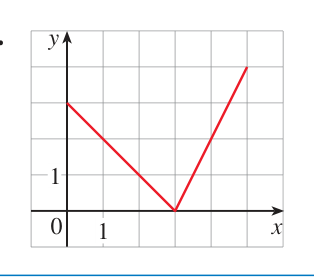
\includegraphics[width=0.82\linewidth]{images/p0055_fig1.png}}
    \end{minipage}%
    \hfill
    \begin{minipage}[t]{0.48\textwidth}
        \textbf{64.}\hfill\raisebox{-\height+1.2ex}{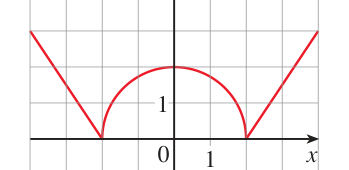
\includegraphics[width=0.82\linewidth]{images/p0055_fig2.png}}
    \end{minipage}

    \vspace{0.66em}
    {\color{stewartcyan}\hrule height 0.6pt}
    \vspace{0.49em}

    \noindent
    \textbf{\textsf{\color{stewartcyan}65--70}}\quad Tìm công thức cho hàm số được mô tả và nêu rõ tập xác định của nó.

    \vspace{0.33em}
    \textbf{65.} Một hình chữ nhật có chu vi $20\text{ m}$. Hãy biểu diễn diện tích của hình chữ nhật theo độ dài một cạnh của nó.

    \vspace{0.25em}
    \textbf{66.} Một hình chữ nhật có diện tích $16\text{ m}^2$. Hãy biểu diễn chu vi của hình chữ nhật theo độ dài một cạnh của nó.

    \vspace{0.25em}
    \textbf{67.} Hãy biểu diễn diện tích của một tam giác đều theo độ dài một cạnh của tam giác.

    \vspace{0.25em}
    \textbf{68.} Một chiếc hộp kín hình hộp chữ nhật có thể tích $8\text{ ft}^3$ và có chiều dài gấp đôi chiều rộng. Hãy biểu diễn chiều cao của chiếc hộp theo chiều rộng.

    \vspace{0.25em}
    \textbf{69.} Một chiếc hộp mở nắp hình hộp chữ nhật có thể tích $2\text{ m}^3$ và có đáy là hình vuông. Hãy biểu diễn diện tích toàn phần của chiếc hộp theo độ dài cạnh đáy.

    \vspace{0.25em}
    \textbf{70.} Một khối trụ tròn xoay có thể tích $25\text{ in}^3$. Hãy biểu diễn bán kính của khối trụ theo chiều cao.

    \vspace{0.66em}
    {\color{stewartcyan}\hrule height 0.6pt}
    \vspace{0.49em}

    \noindent
    \textbf{71.} Một chiếc hộp không nắp được tạo thành từ một tấm bìa các-tông hình chữ nhật có kích thước $12\text{ in.} \times 20\text{ in.}$ bằng cách cắt bỏ các hình vuông bằng nhau có cạnh bằng $x$ ở mỗi góc rồi gấp các mép lên như trong hình vẽ. Hãy biểu diễn thể tích $V$ của chiếc hộp theo $x$.

    \vspace{0.35em}
    \begin{center}
        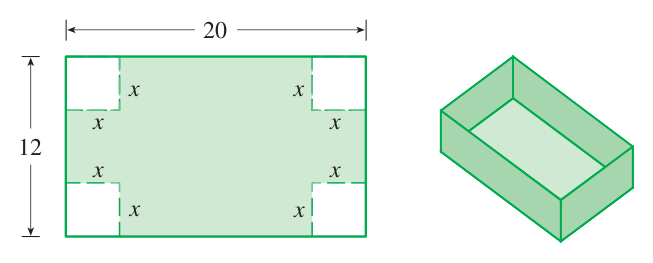
\includegraphics[width=0.92\linewidth]{images/p0055_fig3.png}
    \end{center}

    \vspace{0.35em}
    \noindent
    \textbf{72.} Một cửa sổ Norman có hình dạng gồm một hình chữ nhật bên dưới kết hợp với một nửa hình tròn ở phía trên. Nếu chu vi của cửa sổ là $30\text{ ft}$, hãy biểu diễn diện tích $A$ của cửa sổ theo chiều rộng $x$ của nó.

    \vspace{0.25em}
    \begin{center}
        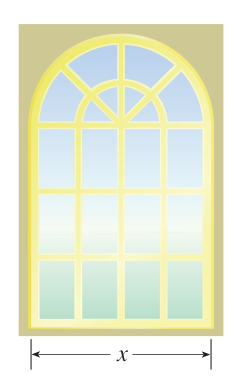
\includegraphics[width=0.35\linewidth]{images/p0055_fig4.png}
    \end{center}

\end{minipage}
\end{document}
